\documentclass[12pt,a4paper]{article}

% ── Packages ────────────────────────────────────────────────────────────────
\usepackage[T1]{fontenc}
\usepackage[utf8]{inputenc}
\usepackage[margin=2.5cm]{geometry}
\usepackage{lmodern}
\usepackage{graphicx}
\usepackage[dvipsnames,table]{xcolor}
\usepackage{booktabs}
\usepackage{tabularx}
\usepackage{array}
\usepackage{enumitem}
\usepackage{listings}
\usepackage{fancyhdr}
\usepackage{titlesec}
\usepackage{amsmath}
\usepackage{tikz}
\usepackage{caption}
\usepackage{hyperref}
\usetikzlibrary{shapes.geometric,arrows.meta,positioning,fit,backgrounds,calc}

% ── Colors ──────────────────────────────────────────────────────────────────
\definecolor{primary}{HTML}{1A3A5C}
\definecolor{accent}{HTML}{2E86AB}
\definecolor{lightgray}{HTML}{F5F5F5}
\definecolor{codebg}{HTML}{F8F9FA}
\definecolor{codeframe}{HTML}{DEE2E6}
\definecolor{green}{HTML}{28A745}
\definecolor{orange}{HTML}{FD7E14}
\definecolor{red}{HTML}{DC3545}
\definecolor{gray}{gray}{0.4}
\definecolor{rowA}{HTML}{EAF4FB}
\definecolor{rowB}{HTML}{FFFFFF}

% ── Hyperref setup ───────────────────────────────────────────────────────────
\hypersetup{
    colorlinks=true,
    linkcolor=primary,
    urlcolor=accent,
    citecolor=accent,
    pdftitle={TahalilAI -- WhatsApp and Email Integration: Feasibility Research},
    pdfauthor={TahalilAI Development Team},
}

% ── Section formatting ───────────────────────────────────────────────────────
\titleformat{\section}
  {\Large\bfseries\color{primary}}
  {\thesection}{1em}{}[\color{accent}\titlerule]

\titleformat{\subsection}
  {\large\bfseries\color{primary}}
  {\thesubsection}{1em}{}

\titleformat{\subsubsection}
  {\normalsize\bfseries\color{primary}}
  {\thesubsubsection}{1em}{}

% ── Header / Footer ──────────────────────────────────────────────────────────
\pagestyle{fancy}
\fancyhf{}
\fancyhead[L]{\small\color{primary}\textbf{TahalilAI}
              \textit{-- Messaging Integration Research}}
\fancyhead[R]{\small\color{primary}March 2026}
\fancyfoot[C]{\small\color{primary}\thepage}
\renewcommand{\headrulewidth}{0.4pt}
\renewcommand{\footrulewidth}{0.4pt}

% ── Code listings ────────────────────────────────────────────────────────────
\lstdefinestyle{python}{
    language=Python,
    backgroundcolor=\color{codebg},
    basicstyle=\ttfamily\footnotesize,
    keywordstyle=\color{accent}\bfseries,
    stringstyle=\color{green!60!black},
    commentstyle=\color{gray}\itshape,
    numberstyle=\tiny\color{gray},
    numbers=left,
    numbersep=8pt,
    frame=single,
    framerule=0.5pt,
    rulecolor=\color{codeframe},
    breaklines=true,
    showstringspaces=false,
    tabsize=4,
    captionpos=b,
    xleftmargin=15pt,
}

\lstdefinestyle{shell}{
    backgroundcolor=\color{black!88},
    basicstyle=\ttfamily\footnotesize\color{white},
    frame=single,
    framerule=0pt,
    breaklines=true,
    showstringspaces=false,
    xleftmargin=10pt,
    xrightmargin=10pt,
}

% ── Custom commands ──────────────────────────────────────────────────────────
\newcommand{\codeinline}[1]{\texttt{\small\color{accent}#1}}

\newcommand{\badge}[2]{%
  \begingroup
  \setlength{\fboxsep}{4pt}%
  \colorbox{#1}{\color{white}\small\textbf{#2}}%
  \endgroup
}

\newcommand{\pro}{\textcolor{green}{\textbf{+}}}
\newcommand{\con}{\textcolor{red}{\textbf{--}}}

% ═════════════════════════════════════════════════════════════════════════════
\begin{document}
% ═════════════════════════════════════════════════════════════════════════════

% ── Title Page ───────────────────────────────────────────────────────────────
\begin{titlepage}
    \centering
    \vspace*{1.8cm}

    {\color{primary}\rule{\linewidth}{2pt}}
    \vspace{0.5cm}

    {\Huge\bfseries\color{primary} TahalilAI}\\[0.3cm]
    {\LARGE\color{accent} Messaging Integration Research}\\[0.2cm]
    {\large\color{gray}
        Feasibility Study: WhatsApp \& Email Delivery of Lab Reports}

    \vspace{0.4cm}
    {\color{primary}\rule{\linewidth}{2pt}}

    \vspace{1.5cm}

    \begin{tabular}{ll}
        \textbf{Project:}       & TahalilAI --- Medical Lab Report Analyzer \\[4pt]
        \textbf{Repository:}    & \href{https://github.com/HealthcareAI-generovo/V1.0}
                                        {HealthcareAI-generovo/V1.0} \\[4pt]
        \textbf{Document type:} & Feasibility Research Report \\[4pt]
        \textbf{Author:}        & TahalilAI Development Team \\[4pt]
        \textbf{Date:}          & March 2026 \\[4pt]
        \textbf{Status:}        & \badge{orange}{DRAFT --- For Supervisor Review} \\
    \end{tabular}

    \vspace{2cm}

    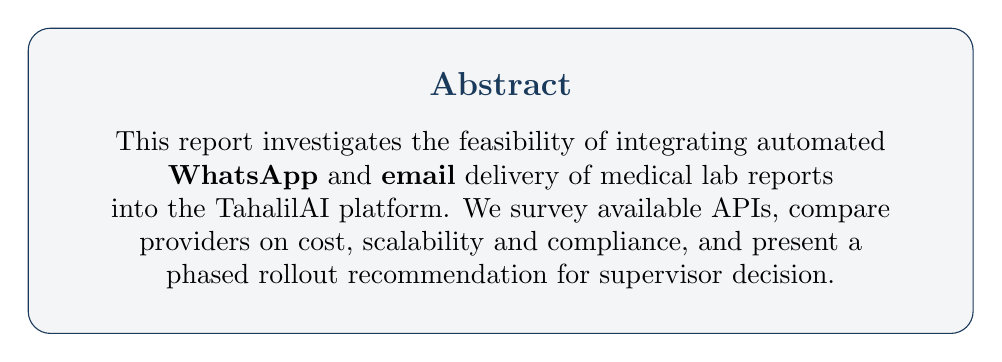
\begin{tikzpicture}
        \node[draw=primary, fill=primary!5, rounded corners=8pt,
              minimum width=12cm, minimum height=3.2cm,
              align=center, inner sep=16pt] {
            \large\color{primary}\textbf{Abstract}\\[8pt]
            \normalsize\color{black}
            This report investigates the feasibility of integrating automated\\
            \textbf{WhatsApp} and \textbf{email} delivery of medical lab reports\\
            into the TahalilAI platform. We survey available APIs, compare\\
            providers on cost, scalability and compliance, and present a\\
            phased rollout recommendation for supervisor decision.
        };
    \end{tikzpicture}

    \vfill
    {\small\color{gray} Internal Research --- Confidential}
\end{titlepage}

\tableofcontents
\newpage

% ═════════════════════════════════════════════════════════════════════════════
\section{Introduction and Motivation}
% ═════════════════════════════════════════════════════════════════════════════

TahalilAI currently delivers lab report analysis exclusively through a web
interface: the patient uploads a file, waits for processing, and views or
downloads the result in-session. While this is functional, it creates a
friction point --- patients must stay on the page or return to retrieve their
report later.

Adding \textbf{push notifications via email and WhatsApp} would allow the
system to proactively deliver results once analysis is complete, improving
patient experience significantly. Both channels are already embedded in the
daily workflows of our target user base across the MENA region.

\subsection{Goals of This Research}

\begin{enumerate}[leftmargin=2em]
    \item Identify the most viable technical approach for each channel.
    \item Assess compliance risk (HIPAA, GDPR, PDPL) for each option.
    \item Compare providers on cost, developer effort, and scalability.
    \item Produce a concrete implementation plan for supervisor approval.
\end{enumerate}

\subsection{Scope}

This study covers outbound notification only (system $\to$ patient). Inbound
messaging (patient replies, chatbot integration) is out of scope for this
iteration.

% ═════════════════════════════════════════════════════════════════════════════
\section{Email Delivery Integration}
% ═════════════════════════════════════════════════════════════════════════════

\subsection{Overview of Approaches}

There are two broad approaches to sending email from TahalilAI's FastAPI
backend: \textbf{(1) direct SMTP} using Python's standard library, and
\textbf{(2) a cloud email API} such as SendGrid or Amazon SES.

% ──────────────────────────────────────────────────────────────────────────
\subsection{Option A --- Gmail SMTP (Prototype Grade)}

Python's built-in \codeinline{smtplib} can connect to Gmail's SMTP server
over TLS/SSL (port 587 STARTTLS or 465 SSL). A 16-digit Gmail App Password
is required; the user's main password does \emph{not} work when 2FA is
enabled.

\begin{lstlisting}[style=python, caption={Minimal Gmail SMTP example (Python)}]
import smtplib
from email.mime.multipart import MIMEMultipart
from email.mime.text import MIMEText
from email.mime.base import MIMEBase
from email import encoders

def send_report_email(patient_email: str, pdf_path: str) -> None:
    msg = MIMEMultipart()
    msg["Subject"] = "Your TahalilAI Lab Report is Ready"
    msg["From"]    = SENDER_EMAIL
    msg["To"]      = patient_email

    body = MIMEText("Please find your lab report attached.", "plain")
    msg.attach(body)

    # Attach PDF
    with open(pdf_path, "rb") as f:
        part = MIMEBase("application", "octet-stream")
        part.set_payload(f.read())
    encoders.encode_base64(part)
    part.add_header("Content-Disposition", f"attachment; filename=report.pdf")
    msg.attach(part)

    with smtplib.SMTP_SSL("smtp.gmail.com", 465) as server:
        server.login(SENDER_EMAIL, APP_PASSWORD)
        server.sendmail(SENDER_EMAIL, [patient_email], msg.as_string())
\end{lstlisting}

\noindent\textbf{Assessment:}
\begin{itemize}[leftmargin=2em, itemsep=2pt]
    \item[\pro] Zero cost, zero new dependencies, fastest to prototype.
    \item[\con] A free Gmail account is \textbf{not HIPAA-compliant}. No BAA
          available without Google Workspace (paid).
    \item[\con] Rate-limited to ~500 recipients/day for free accounts.
    \item[\con] No built-in delivery tracking, bounce handling, or analytics.
\end{itemize}

% ──────────────────────────────────────────────────────────────────────────
\subsection{Option B --- SendGrid / AWS SES (Production Grade)}

Cloud email APIs provide better reliability, deliverability infrastructure
(SPF/DKIM/DMARC managed), and compliance tooling.

\begin{table}[h!]
\centering
\begin{tabularx}{\linewidth}{l X X}
\toprule
\textbf{Provider} & \textbf{Free Tier} & \textbf{Key Features} \\
\midrule
\rowcolor{rowA}
\textbf{SendGrid} (Twilio) &
    100 emails/day free &
    REST API, Python SDK, webhooks, HIPAA BAA available on higher plans \\
\textbf{AWS SES} &
    62,000 emails/mo free (from EC2) &
    Very low cost (\$0.10/1000), BAA available in covered accounts,
    deep AWS integration \\
\rowcolor{rowA}
\textbf{Mailgun} &
    100 emails/day (5000/mo for 3 months) &
    Python SDK, detailed logs, HIPAA BAA available \\
\textbf{Postmark} &
    100 emails/mo free &
    High deliverability focus, transactional email specialist \\
\bottomrule
\end{tabularx}
\caption{Cloud email provider comparison}
\end{table}

\begin{lstlisting}[style=python, caption={SendGrid API email (Python SDK)}]
import sendgrid
from sendgrid.helpers.mail import Mail, Attachment, FileContent, FileName
import base64

def send_via_sendgrid(patient_email: str, pdf_bytes: bytes) -> None:
    sg = sendgrid.SendGridAPIClient(api_key=SENDGRID_API_KEY)

    message = Mail(
        from_email="reports@tahalilai.com",
        to_emails=patient_email,
        subject="Your TahalilAI Lab Report is Ready",
        html_content="<p>Your analysis is complete. See attached PDF.</p>",
    )
    attachment = Attachment(
        FileContent(base64.b64encode(pdf_bytes).decode()),
        FileName("lab_report.pdf"),
    )
    message.attachment = attachment
    sg.send(message)
\end{lstlisting}

\noindent\textbf{Assessment:}
\begin{itemize}[leftmargin=2em, itemsep=2pt]
    \item[\pro] Deliverability infrastructure (SPF, DKIM, DMARC) managed.
    \item[\pro] BAA available on SendGrid Pro/AWS SES --- HIPAA-compatible.
    \item[\pro] Webhooks for delivery receipts, bounces, unsubscribes.
    \item[\con] Cost above free tier; requires domain verification.
\end{itemize}

% ──────────────────────────────────────────────────────────────────────────
\subsection{Email Content and Format}

Regardless of the transport layer, the email should:

\begin{itemize}[leftmargin=2em, itemsep=2pt]
    \item Use an HTML template with the TahalilAI branding.
    \item Include the \textbf{AI summary} in plain text in the body.
    \item Attach the \textbf{generated PDF report} (already produced by the
          existing pipeline).
    \item Provide a \textbf{secure portal link} for viewing full results
          online when PHI transmission over email is restricted.
    \item Include a one-click \textbf{unsubscribe link} to comply with
          anti-spam legislation (CAN-SPAM, GDPR).
\end{itemize}

% ═════════════════════════════════════════════════════════════════════════════
\section{WhatsApp Messaging Integration}
% ═════════════════════════════════════════════════════════════════════════════

\subsection{Overview}

WhatsApp is the dominant messaging platform in the MENA region, with over
2 billion monthly users globally. Delivery and open rates far exceed email
for mobile-first populations. However, business use requires compliance with
Meta's policies, and healthcare PHI transmission introduces regulatory risk.

There are two primary integration paths: the \textbf{Official WhatsApp Cloud
API} (Meta-hosted), or a \textbf{third-party CPaaS provider} such as Twilio
or 360dialog that acts as a Meta Business Solution Provider (BSP).

% ──────────────────────────────────────────────────────────────────────────
\subsection{Option A --- WhatsApp Cloud API (Official, Meta-Hosted)}

Meta's Cloud API allows our server to send and receive WhatsApp messages
directly via HTTPS calls to the Graph API. No self-hosted infrastructure is
required; Meta manages the messaging layer.

\textbf{Setup requirements:}
\begin{enumerate}[leftmargin=2em, itemsep=2pt]
    \item Create a Meta Developer account and a Business Manager.
    \item Register a dedicated phone number for WhatsApp Business.
    \item Create a WhatsApp Business App in Meta's Developer Portal.
    \item Submit and get approved at least one message template.
    \item Configure a public HTTPS webhook to receive inbound events.
\end{enumerate}

\begin{lstlisting}[style=python, caption={Meta Cloud API: send a template message (Python/requests)}]
import requests

PHONE_NUMBER_ID = "your_phone_number_id"
ACCESS_TOKEN    = "your_meta_api_token"

def send_whatsapp_notification(to_number: str) -> dict:
    url = (
        f"https://graph.facebook.com/v19.0/"
        f"{PHONE_NUMBER_ID}/messages"
    )
    headers = {
        "Authorization": f"Bearer {ACCESS_TOKEN}",
        "Content-Type":  "application/json",
    }
    payload = {
        "messaging_product": "whatsapp",
        "to": to_number,          # international format, e.g. "213XXXXXXXXX"
        "type": "template",
        "template": {
            "name": "lab_report_ready",
            "language": {"code": "en_US"},
            "components": [
                {
                    "type": "body",
                    "parameters": [
                        {"type": "text", "text": "TahalilAI"}
                    ],
                }
            ],
        },
    }
    response = requests.post(url, headers=headers, json=payload)
    return response.json()
\end{lstlisting}

\noindent\textbf{Messaging windows and templates:}

Meta enforces two conversation modes:
\begin{itemize}[leftmargin=2em, itemsep=2pt]
    \item \textbf{Business-initiated} (outside 24h window): must use a
          pre-approved template. Templates are reviewed by Meta (typically
          under 24 hours). Categories: \emph{Marketing}, \emph{Utility},
          \emph{Authentication}.
    \item \textbf{Service messages} (within 24h of a user message): free-form
          text is allowed. Not applicable for outbound-only notifications.
\end{itemize}

\noindent\textbf{Assessment:}
\begin{itemize}[leftmargin=2em, itemsep=2pt]
    \item[\pro] No middleman; lowest per-message cost at scale.
    \item[\pro] Official SDK (Graph API), very stable and well-documented.
    \item[\con] Setup is lengthy; Meta app review can take days.
    \item[\con] Requires public HTTPS webhook for status callbacks.
    \item[\con] \textbf{No HIPAA BAA available from Meta.}
\end{itemize}

% ──────────────────────────────────────────────────────────────────────────
\subsection{Option B --- Twilio WhatsApp API (CPaaS / BSP)}

Twilio acts as a Meta Business Solution Provider, abstracting the Graph API
behind a simpler REST interface and Python SDK. Twilio also offers a
\textbf{free sandbox} for development that requires no Meta approval.

\begin{lstlisting}[style=python, caption={Twilio WhatsApp message (Python SDK)}]
from twilio.rest import Client

def send_via_twilio(to_number: str) -> None:
    client = Client(TWILIO_ACCOUNT_SID, TWILIO_AUTH_TOKEN)
    message = client.messages.create(
        from_="whatsapp:+14155238886",   # Twilio sandbox / your number
        to=f"whatsapp:{to_number}",
        body=(
            "Your TahalilAI lab report is ready. "
            "Please log in to your portal to view your results."
        ),
    )
    print(f"Message SID: {message.sid}")
\end{lstlisting}

\noindent\textbf{Pricing (Twilio, as of 2026):}
\begin{itemize}[leftmargin=2em, itemsep=2pt]
    \item Outbound template (utility): \textbf{\$0.005/message} + Meta's
          per-conversation fee ($\sim$\$0.02--\$0.08 depending on country).
    \item Algeria (DZD market): approximately \$0.04--\$0.06 per conversation.
    \item Free trial includes \$15 credits --- sufficient for hundreds of
          test messages.
\end{itemize}

\noindent\textbf{Assessment:}
\begin{itemize}[leftmargin=2em, itemsep=2pt]
    \item[\pro] Fastest developer onboarding; sandbox available immediately.
    \item[\pro] Excellent Python SDK, webhooks, and delivery analytics.
    \item[\pro] Twilio signs a HIPAA BAA --- shifts some compliance burden.
    \item[\con] Extra cost layer (Twilio margin) on top of Meta fees.
    \item[\con] At high volume, the Cloud API directly is cheaper.
\end{itemize}

% ──────────────────────────────────────────────────────────────────────────
\subsection{Option C --- 360dialog}

360dialog is a European BSP that provides a UI-driven onboarding to the
official Cloud API, with a flat monthly fee (\$\sim$49/month) rather than
per-message pricing. This model is cost-effective for high volume. Worth
considering if the pilot is successful.

% ──────────────────────────────────────────────────────────────────────────
\subsection{WhatsApp Use Case Constraints}

A critical design constraint: \textbf{WhatsApp is not HIPAA-compliant.} Meta
does not sign Business Associate Agreements. Therefore:

\begin{itemize}[leftmargin=2em, itemsep=2pt]
    \item WhatsApp messages must \textbf{not} contain raw PHI (lab values,
          diagnoses, patient IDs).
    \item The safe pattern is a \textbf{minimal alert}: ``Your TahalilAI
          report is ready. Please check your email or log into the portal.''
    \item The full PDF report and AI analysis should be delivered via email
          or the secure web portal.
    \item Patient \textbf{opt-in consent} must be obtained before any
          WhatsApp message is sent.
\end{itemize}

% ═════════════════════════════════════════════════════════════════════════════
\section{Compliance and Privacy Considerations}
% ═════════════════════════════════════════════════════════════════════════════

\subsection{Regulatory Landscape}

The TahalilAI platform processes Protected Health Information (PHI) and is
subject to multiple overlapping frameworks depending on deployment region:

\begin{table}[h!]
\centering
\begin{tabularx}{\linewidth}{l X X}
\toprule
\textbf{Regulation} & \textbf{Jurisdiction} & \textbf{Key Requirement} \\
\midrule
\rowcolor{rowA}
HIPAA (Health Insurance Portability and Accountability Act) &
    United States &
    PHI must be encrypted in transit and at rest; BAA required with
    all vendors handling PHI \\
GDPR (General Data Protection Regulation) &
    European Union &
    Explicit consent for personal data processing; right to erasure;
    data minimisation \\
\rowcolor{rowA}
PDPL (Personal Data Protection Law) &
    Saudi Arabia &
    Data localisation requirements; consent for health data;
    breach notification within 72h \\
UAE Health Data Law &
    UAE &
    Health data must stay in UAE data centres unless explicit consent \\
\bottomrule
\end{tabularx}
\caption{Applicable data protection regulations}
\end{table}

\subsection{Compliance Matrix by Channel}

\begin{table}[h!]
\centering
\rowcolors{2}{rowA}{rowB}
\begin{tabularx}{\linewidth}{l >{\centering\arraybackslash}X >{\centering\arraybackslash}X >{\centering\arraybackslash}X}
\toprule
\textbf{Criterion} &
    \textbf{Gmail SMTP} &
    \textbf{SendGrid / SES} &
    \textbf{WhatsApp (any)} \\
\midrule
HIPAA BAA available &
    \textcolor{red}{No (free)} / \textcolor{green}{Yes (Workspace)} &
    \textcolor{green}{Yes} &
    \textcolor{red}{No (Meta)} / \textcolor{green}{Twilio BAA} \\
Encryption in transit &
    \textcolor{green}{TLS} &
    \textcolor{green}{TLS} &
    \textcolor{green}{E2E (device)} \\
PHI safe to transmit &
    \textcolor{orange}{With BAA only} &
    \textcolor{green}{Yes (with BAA)} &
    \textcolor{red}{No (no Meta BAA)} \\
Consent mechanism &
    Email opt-in required &
    Email opt-in required &
    Explicit WhatsApp opt-in \\
Audit trail &
    \textcolor{orange}{Manual logging} &
    \textcolor{green}{Built-in webhooks} &
    \textcolor{orange}{Twilio logs only} \\
\bottomrule
\end{tabularx}
\caption{Compliance comparison across channels}
\end{table}

\subsection{Patient Consent Implementation}

An opt-in flow must be implemented in the user registration or settings
screen:

\begin{enumerate}[leftmargin=2em, itemsep=2pt]
    \item Patient enters email and/or WhatsApp number.
    \item A checkbox (unchecked by default) reads: ``I consent to receiving
          my lab report notifications via [email / WhatsApp].''
    \item Consent timestamp and channel are stored in the database.
    \item A \textbf{revoke consent} button is accessible from the profile
          page at any time.
    \item WhatsApp requires an additional step: the patient must send a
          first message from their number to our WhatsApp Business number
          to initiate the conversation window (Meta policy).
\end{enumerate}

\subsection{Data Minimisation for WhatsApp}

Given the absence of a Meta BAA, WhatsApp messages must apply strict data
minimisation:

\begin{itemize}[leftmargin=2em]
    \item \textbf{Allowed}: patient first name, date, portal link.
    \item \textbf{Prohibited}: lab values, diagnoses, medications, report
          content, patient ID numbers.
\end{itemize}

% ═════════════════════════════════════════════════════════════════════════════
\section{Technical Architecture}
% ═════════════════════════════════════════════════════════════════════════════

\subsection{System Flow}

When the TahalilAI analysis pipeline completes, the backend enqueues a
notification job. A background worker resolves the patient's opted-in
channels and dispatches accordingly.

\begin{center}
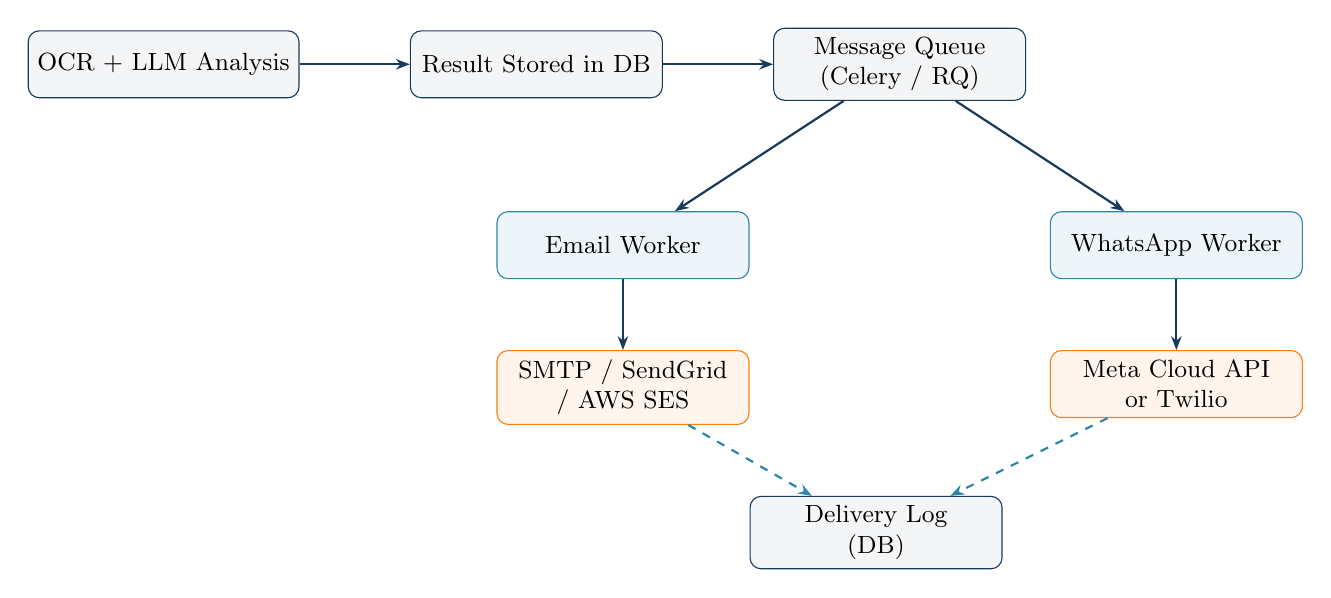
\begin{tikzpicture}[
    node distance=0.9cm and 1.4cm,
    box/.style={draw=primary, fill=primary!5, rounded corners=4pt,
                minimum width=3.2cm, minimum height=0.85cm, align=center,
                font=\small},
    worker/.style={draw=accent, fill=accent!8, rounded corners=4pt,
                   minimum width=3.2cm, minimum height=0.85cm, align=center,
                   font=\small},
    ext/.style={draw=orange, fill=orange!8, rounded corners=4pt,
                minimum width=3.2cm, minimum height=0.85cm, align=center,
                font=\small},
    decision/.style={draw=orange, fill=orange!8, diamond, aspect=2.2,
                     minimum width=3cm, minimum height=0.7cm, align=center,
                     font=\footnotesize},
    arrow/.style={-{Stealth[length=5pt]}, thick, color=primary},
    darrow/.style={-{Stealth[length=5pt]}, thick, color=accent, dashed},
]
    \node[box]      (ocr)    {OCR + LLM Analysis};
    \node[box, right=1.4cm of ocr]   (db)   {Result Stored in DB};
    \node[box, right=1.4cm of db]    (queue){Message Queue\\(Celery / RQ)};

    \node[worker, below left=1.4cm and 0.3cm of queue]  (ew)  {Email Worker};
    \node[worker, below right=1.4cm and 0.3cm of queue] (ww)  {WhatsApp Worker};

    \node[ext, below=0.9cm of ew]   (smtp)  {SMTP / SendGrid\\/ AWS SES};
    \node[ext, below=0.9cm of ww]   (wa)    {Meta Cloud API\\or Twilio};

    \node[box, below right=0.9cm and 0cm of smtp] (log) {Delivery Log\\(DB)};

    \draw[arrow] (ocr)   -- (db);
    \draw[arrow] (db)    -- (queue);
    \draw[arrow] (queue) -- (ew);
    \draw[arrow] (queue) -- (ww);
    \draw[arrow] (ew)    -- (smtp);
    \draw[arrow] (ww)    -- (wa);
    \draw[darrow] (smtp) -- (log);
    \draw[darrow] (wa)   -- (log);
\end{tikzpicture}
\end{center}

\subsection{Tech Stack Summary}

\begin{table}[h!]
\centering
\begin{tabularx}{\linewidth}{l l X}
\toprule
\textbf{Layer} & \textbf{Technology} & \textbf{Role} \\
\midrule
\rowcolor{rowA}
Web Framework & FastAPI (existing) &
    REST endpoints, background task scheduling \\
Task Queue & Celery + Redis \emph{or} FastAPI \codeinline{BackgroundTasks} &
    Asynchronous message dispatch without blocking the HTTP response \\
\rowcolor{rowA}
Email (dev) & \codeinline{smtplib} / \codeinline{fastapi-mail} &
    Rapid prototyping with Gmail App Password \\
Email (prod) & SendGrid Python SDK \emph{or} \codeinline{boto3} (SES) &
    Reliable delivery, bounce handling, HIPAA BAA \\
\rowcolor{rowA}
WhatsApp (dev) & Twilio Python SDK + Sandbox &
    Instant setup, no Meta approval needed \\
WhatsApp (prod) & Meta Graph API (\codeinline{requests}) \emph{or} Twilio &
    Official integration, approved templates \\
\rowcolor{rowA}
Database & Existing DB (PostgreSQL / SQLite) &
    Consent flags, contact info, delivery log \\
Secrets & Environment variables / \codeinline{.env} &
    API keys, SMTP credentials (never hardcoded) \\
\bottomrule
\end{tabularx}
\caption{Proposed messaging tech stack}
\end{table}

\subsection{New Database Fields}

Two additions to the \codeinline{patients} (or \codeinline{users}) table:

\begin{lstlisting}[style=python, caption={Pydantic schema additions (example)}]
class PatientNotificationPrefs(BaseModel):
    email: str | None = None
    email_consent: bool = False
    email_consent_at: datetime | None = None

    whatsapp_number: str | None = None          # E.164 format
    whatsapp_consent: bool = False
    whatsapp_consent_at: datetime | None = None
\end{lstlisting}

A separate \codeinline{delivery\_log} table tracks:

\begin{lstlisting}[style=python, caption={Delivery log schema (example)}]
class DeliveryLog(BaseModel):
    job_id: str           # links to analysis job
    channel: str          # "email" | "whatsapp"
    status: str           # "pending" | "sent" | "failed"
    provider_message_id: str | None = None
    sent_at: datetime | None = None
    error: str | None = None
\end{lstlisting}

\subsection{FastAPI Integration Points}

Three minimal additions to the existing \codeinline{app.py}:

\begin{enumerate}[leftmargin=2em, itemsep=2pt]
    \item \textbf{POST \codeinline{/notify/email}} --- manually trigger an
          email for a completed job (or triggered automatically inside
          \codeinline{\_run\_pipeline}).
    \item \textbf{POST \codeinline{/notify/whatsapp}} --- trigger a WhatsApp
          notification for a completed job.
    \item \textbf{POST \codeinline{/webhook/whatsapp}} --- public endpoint to
          receive Meta/Twilio delivery receipts and status updates.
\end{enumerate}

% ═════════════════════════════════════════════════════════════════════════════
\section{Provider Comparison and Decision Matrix}
% ═════════════════════════════════════════════════════════════════════════════

\begin{table}[h!]
\centering
\rowcolors{2}{rowA}{rowB}
\begin{tabularx}{\linewidth}{l
    >{\centering\arraybackslash}X
    >{\centering\arraybackslash}X
    >{\centering\arraybackslash}X
    >{\centering\arraybackslash}X}
\toprule
\textbf{Criterion} &
    \textbf{Gmail SMTP} &
    \textbf{SendGrid} &
    \textbf{WA Cloud API} &
    \textbf{Twilio WA} \\
\midrule
Cost &
    Free &
    Free--\$19.95/mo &
    Meta fees only &
    Meta + \$0.005/msg \\
Setup effort &
    \badge{green}{Low} &
    \badge{green}{Low} &
    \badge{red}{High} &
    \badge{orange}{Medium} \\
Dev sandbox &
    \textcolor{green}{\checkmark} &
    \textcolor{green}{\checkmark} &
    \textcolor{red}{\texttimes} &
    \textcolor{green}{\checkmark} \\
HIPAA BAA &
    \textcolor{red}{No (free)} &
    \textcolor{green}{Yes (paid)} &
    \textcolor{red}{No} &
    \textcolor{green}{Yes (Twilio)} \\
PHI in message &
    With BAA &
    With BAA &
    \textcolor{red}{No} &
    \textcolor{red}{No (Meta)} \\
Scalability &
    \badge{orange}{Limited} &
    \badge{green}{High} &
    \badge{green}{High} &
    \badge{green}{High} \\
Analytics &
    \textcolor{red}{None} &
    \textcolor{green}{Full} &
    \textcolor{orange}{Webhooks} &
    \textcolor{green}{Full} \\
MENA reach &
    Universal &
    Universal &
    \textcolor{green}{\textbf{Very high}} &
    \textcolor{green}{\textbf{Very high}} \\
\bottomrule
\end{tabularx}
\caption{Full provider decision matrix}
\end{table}

\subsection{Recommended Stack}

Based on the matrix above, the recommended configuration is:

\begin{itemize}[leftmargin=2em]
    \item \textbf{Email (PHI delivery)}: \badge{green}{SendGrid}
          with HIPAA BAA, or AWS SES inside a HIPAA-covered account.
          Attach the full PDF report. Authenticate the domain with
          SPF/DKIM/DMARC.
    \item \textbf{WhatsApp (alert only)}: \badge{accent}{Twilio WhatsApp}
          for the pilot phase (sandbox → production). Message content
          restricted to a non-PHI notification. Twilio's BAA is available
          even if Meta's is not.
    \item \textbf{Long-term WhatsApp at scale}: Migrate to the
          \badge{primary}{Meta Cloud API} directly once usage justifies
          eliminating Twilio's margin.
\end{itemize}

% ═════════════════════════════════════════════════════════════════════════════
\section{Phased Rollout Plan}
% ═════════════════════════════════════════════════════════════════════════════

\begin{table}[h!]
\centering
\begin{tabularx}{\linewidth}{l l X}
\toprule
\textbf{Phase} & \textbf{Timeline} & \textbf{Deliverables} \\
\midrule
\rowcolor{rowA}
\textbf{1 --- Email Prototype} & Week 1--2 &
    Implement Gmail SMTP sending from \codeinline{\_run\_pipeline}.
    Email with AI summary + PDF attachment. Delivery log in DB.
    Internal testing only. \\
\textbf{2 --- Email Production} & Week 3--4 &
    Switch to SendGrid (or SES). Configure domain authentication
    (SPF, DKIM, DMARC). Sign BAA. HTML email template. Opt-in
    consent UI. Unsubscribe link. \\
\rowcolor{rowA}
\textbf{3 --- WhatsApp Sandbox} & Week 3--5 &
    Integrate Twilio sandbox. Draft and test template messages.
    Add consent field to patient profile. Webhook endpoint for
    delivery receipts. Internal QA. \\
\textbf{4 --- Compliance Review} & Week 5--6 &
    Legal/compliance review of message content and consent flows.
    Define PHI exclusion rules for WhatsApp. Document consent
    process for GDPR/PDPL records. \\
\rowcolor{rowA}
\textbf{5 --- Pilot Launch} & Month 2 &
    Invite small opt-in cohort. Send WhatsApp alerts (non-PHI) and
    full email reports. Monitor delivery rates, open rates,
    patient feedback. \\
\textbf{6 --- Full Deployment} & Month 3+ &
    Graduate Twilio to production number (approved templates).
    Assess volume --- migrate to Meta Cloud API if $>$10k messages/month.
    Continuous monitoring and cost review. \\
\bottomrule
\end{tabularx}
\caption{Phased rollout timeline}
\end{table}

% ═════════════════════════════════════════════════════════════════════════════
\section{Risk Assessment}
% ═════════════════════════════════════════════════════════════════════════════

\begin{table}[h!]
\centering
\rowcolors{2}{rowA}{rowB}
\begin{tabularx}{\linewidth}{X >{\centering\arraybackslash}p{2cm}
    >{\centering\arraybackslash}p{2cm} X}
\toprule
\textbf{Risk} & \textbf{Likelihood} & \textbf{Severity} & \textbf{Mitigation} \\
\midrule
PHI exposed in WhatsApp message &
    Medium & \textcolor{red}{High} &
    Strict content rules; non-PHI templates only; legal review \\
Meta template rejection (delays) &
    Medium & Medium &
    Twilio sandbox for development; submit templates early \\
Email marked as spam &
    Low & Medium &
    Domain authentication (SPF/DKIM/DMARC); reputable provider \\
Regulatory non-compliance (PDPL) &
    Low & \textcolor{red}{High} &
    Consent logging; regional data residency; legal sign-off \\
Twilio/SendGrid outage &
    Very low & Medium &
    Fallback to SMTP; retry queue with exponential backoff \\
Patient opt-out ignored &
    Very low & \textcolor{red}{High} &
    Preference DB enforced at dispatch; automated suppression list \\
\bottomrule
\end{tabularx}
\caption{Risk register}
\end{table}

% ═════════════════════════════════════════════════════════════════════════════
\section{Cost Estimate}
% ═════════════════════════════════════════════════════════════════════════════

Assuming \textbf{500 patients/month}, each receiving one email and one
WhatsApp alert:

\begin{table}[h!]
\centering
\begin{tabularx}{\linewidth}{l X >{\centering\arraybackslash}p{3cm}}
\toprule
\textbf{Item} & \textbf{Details} & \textbf{Est. Monthly Cost} \\
\midrule
\rowcolor{rowA}
SendGrid Essentials & 50,000 emails/mo plan & \$19.95 \\
Twilio WhatsApp & 500 msgs $\times$ \$0.005 + Meta fees $\approx$
    500 $\times$ \$0.06 & $\sim$\$33 \\
\rowcolor{rowA}
Redis (task queue) & Managed Redis (Upstash free tier) & \$0 \\
Domain email auth & One-time DNS setup & \$0 \\
\midrule
\textbf{Total} & & \textbf{$\sim$\$53/month} \\
\bottomrule
\end{tabularx}
\caption{Estimated monthly cost at 500 patients/month}
\end{table}

At 5,000 patients/month the cost scales linearly to approximately
\textbf{\$250--\$300/month}. Migrating WhatsApp to the Cloud API directly
reduces the Twilio margin and would lower the cost by $\sim$30\% at that
volume.

% ═════════════════════════════════════════════════════════════════════════════
\section{Conclusion and Recommendation}
% ═════════════════════════════════════════════════════════════════════════════

Both email and WhatsApp integration are technically feasible within the
existing FastAPI architecture of TahalilAI. The principal findings of this
research are:

\begin{enumerate}[leftmargin=2em, itemsep=4pt]
    \item \textbf{Email is the primary delivery channel for full reports.}
          With a HIPAA BAA from SendGrid or AWS SES, it is safe to transmit
          the complete PDF analysis. Setup effort is low, cost is minimal,
          and patient familiarity is universal.

    \item \textbf{WhatsApp is best used as a lightweight alert channel.}
          Its high open rates and regional penetration make it excellent
          for notifying patients that their report is ready. However,
          because Meta does not sign HIPAA BAAs, the message content must
          be strictly non-PHI. The actual report must remain on a secure
          channel (email or portal).

    \item \textbf{Twilio is the recommended WhatsApp provider for the pilot.}
          The sandbox removes the Meta approval bottleneck during
          development, the Python SDK is clean and well-documented, and
          Twilio does offer its own HIPAA BAA to partially cover
          infrastructure compliance.

    \item \textbf{The rollout can begin immediately.} Phase 1 (email
          prototype) requires no new accounts or approvals --- only the
          existing \codeinline{smtplib} library and a Gmail App Password.
          The entire six-phase plan can be completed within three months.
\end{enumerate}

\vspace{1em}
\noindent\textbf{Decision requested from supervisor:}

\begin{itemize}[leftmargin=2em]
    \item Approve Phase 1 (email prototype) to begin immediately?
    \item Approve signing a SendGrid or AWS SES BAA for production email?
    \item Authorise a Twilio account for WhatsApp sandbox development?
    \item Initiate legal/compliance review for GDPR/PDPL consent flows?
\end{itemize}

\vspace{2em}
\hrule
\vspace{0.8em}
{\small\color{gray}
Prepared by the TahalilAI Development Team --- March 2026.
This document is a feasibility study intended for internal review.
All cost figures are estimates based on public provider pricing pages
at the time of writing and are subject to change.
}

\end{document}
